\documentclass[10pt,oneside,a4paper]{article}

\usepackage{hyperref}
\usepackage{graphicx}
\usepackage{amsmath}
\newif\ifincludeimages

\includeimagestrue 
%\includeimagesfalse
\hypersetup{
	colorlinks=true,   % Abilita il colore dei link (senza box intorno)
	linkcolor=blue,    % Colore per i link interni (come quelli nell'indice)
	urlcolor=red,      % Colore per i link URL esterni
	filecolor=magenta, % Colore per i link ai file locali
	citecolor=green,   % Colore per i riferimenti bibliografici
	pdfborder={0 0 0}  % Disabilita i bordi intorno ai link
}
\title{Introduzione all'apprendimento automatico}
\author{Matteo Mazzaretto, Davide Lorenzon}
\date{2024/2025}
\begin{document}
\pagenumbering{gobble}
\maketitle
\begin{center}
%do un nuovo nome alla tabella degli indici e la inizializzo
\renewcommand{\contentsname}{Indice}
\tableofcontents
\end{center}
\newpage
%inizio l'effettivo conteggio delle pagine
\pagenumbering{arabic}
\setcounter{page}{1}
\section{Prima parte}
\subsection{Si descrivano nel modo più accurato possibile i concetti di bias e variance, il loro rapporto e come nella pratica possano essere affrontati e ridotti i problemi. A tal fine si riportino anche esempi concreti che aiutino a chiarire i diversi aspetti coinvolti}
Il bias rappresenta l'errore sistematico introdotto da un modello nel semplificare troppo il problema, portando a una rappresentazione inaccurata dei dati\\
L'inductive bias rappresenta l'insieme di ipotesi che un algoritmo assume sulla funzione target per poter generalizzare dai dati di training ai dati nuovi\\
Infatti, nel caso della regressione lineare, l'inductive bias principale è che l'insieme di input e output può essere rappresentato come una funzione lineare\\
Ci sono esattamente due tipi:
\begin{enumerate}
	\item restriction: limita lo spazio delle ipotesi
	\item impone l'ordine delle preferenze
\end{enumerate}
Il bias alto causa all'algoritmo la mancanza di relazioni rilevanti fra feature e target, ad esempio un modello di regressione lineare ha un bias alto se i dati reali seguono una relazione quadratica: la sua rigidità lo porterà a fare errori sistematici.
La variance misura quanto il modello è sensibile alle variazioni nei dati di training\\
Un modello ha varianza alta quando è molto sensibile ai cambiamenti nei dati di training: piccole variazioni nei dati possono portare a grandi differenze nelle predizioni\\
Questo accade quando il modello è troppo complesso e tende a sovradattarsi (overfitting)\\
Il loro rapporto principale porta al bias-variance tradeoff, ovvero ciò che rappresenta il rapporto tra bias e varianza: un modello con bias alto semplifica troppo il problema (underfitting), mentre un modello con varianza alta si adatta troppo ai dati di training (overfitting)\\
L'obiettivo è trovare un equilibrio tra i due per minimizzare l'errore totale\\
La cosa migliore per un algoritmo sarebbe avere bias basso, varianza bassa\\
Alcuni metodi pratici per bilanciare bias e varianza:\\
1) Ridurre il bias: usare modelli più complessi (es. passare da regressione lineare a polinomiale)\\
2) Ridurre la varianza: usare più dati di training\\
Diverse tecniche di apprendimento hanno diversi tipi di inductive bias:\\
\begin{enumerate}
	\item Regressione Lineare: assume che la relazione tra input e output sia lineare. Se i dati seguono una relazione non lineare, il modello farà errori sistematici
	\item Reti Neurali: hanno un bias più flessibile, ma la loro architettura impone certe strutture (es. una rete convoluzionale è adatta a dati con correlazioni spaziali, come immagini)
	\item Nearest Neighbors (NN): assume che dati simili abbiano etichette simili, basandosi sulla vicinanza in uno spazio di feature
\end{enumerate}


\subsection{Concetti principali}
\subsubsection{Linear Regression}
la regressione lineare è una delle tecniche fondamentali nella \textbf{creazione di learning algorithms}.\\
Ci permette, dato un set di dati di training composto da dei dati di ''input'' con una o più features e un dato target, di individuare una funzione approsimante del dataset che permetta di trovare il valore target anche per dati esterni al set di training. \\
Per fare ciò useremo le seguenti funzioni:
\begin{itemize}
 \item la seguente funzione permette, dato un input con una o più feature, di calcolare il target :
  $$h_{\Theta}(x)=\Theta_{0}+\Theta_{1}x_1$$
  \textbf{Nota Bene}: in questo esempio il dato di input ha solo una feature, quindi abbiamo solo una variabile ($ x_1$ )\\
 Nella formula precedente i $\Theta_{i}$ rappresentano dei coefficienti o pesi che cercano di realizzare una funzione tale che 
 $$h_{\Theta}(x^{(i)})\approx y^{(i)}  \forall i$$
 Le varie feature vanno pesate in quanto non contribuiscono in maniera omogenea al risultato (una caratteristica può essere più rilevante delle altre)
 \item La seguente funzione è detta \textbf{funzione di costo} è:
 $$J(\Theta_{0},\Theta_{1})= \frac{1}{2m} \sum_{i=1}^{m}(h_{\Theta}(x^{(i)})-y^{(i)})^2$$
 \item Il nostro obiettivo è \textbf{ minimizzare }la funzione di costo
 $$\min_{\Theta_{0},\Theta_{1}} J(\Theta_{0},\Theta_{1})$$
 
 \end{itemize}
 
 \subsubsection{Parameter learning, Gradient descend}
Al fine di minimizzare la funzione di costo ci serve un algoritmo efficiente per aggiustare automaticamente i parametri $\Theta$ \\
Per fare ciò usiamo il \textbf{Gradient descend} 
 \begin{itemize}
\item Data una funzione di costo:
$$J(\Theta_{0},......,\Theta_{n})$$
\item facciamo un piccolo ``passo'' nella direzione opposta al gradiente (gradiente moltiplicato per $-1$), si noti che questo algoritmo porta ad un minimo locale e potrebbe differire in base al punto di partenza (si veda figura 2)
$$\Theta^{(j+1)} = \Theta^{(j)}-\eta \nabla J(\Theta^{(j)})$$
Volendo fare un'analogia per chiarire il concetto possiamo immaginare di trovarci in montagna con una nebbia molto fitta, per tornare a valle cerchiamo di fare sempre un passo in discesa (si veda figura 1)



\item $\Theta^{(j)}$ indica l'insieme delle $\Theta_{0},......,\Theta_{n}$ al j esimo passo \\
(\textbf{NB} se l'aggiornamento delle $\theta $ non avviene come operazioni tra vettori, ma considerando ogni $\Theta$ come uno scalare è necessario aggiungere delle variabili temporanee per evitare che i cambiamenti di un $\Theta$ inluenzi anche gli altri)

\item $\eta > 0$ è chiamato \textbf{learning rate}, è importante che non sia un valore troppo basso, perchè potrebbe portare a una convergenza troppo lenta, è importante che non sia troppo alto, perchè potrebbe non convergere (figura 3)

\item dopo ogni passaggio il gradiente viene rivalutato per il nuovo vettore dei pesi $\Theta^{(j+1)}$ 
\\ il processo si ripete finchè non si raggiunge uno scarto sufficientemente basso (il criterio dello scarto ferma la discesa del gradiente quando la differenza tra il gradiente al passo j e j+1 è prossima a 0 )

\item  \textbf{Nota bene}: la funzione di costo va calcolata sull'interezza dei dati di addestramento gli x e y, \\
in particolare X diventa matrice e Y diventa vettore (batch gradient descend)
$$\nabla J(\Theta)=\frac{1}{m}X^{T}(h_{\Theta}(X)-Y)$$
 \begin{itemize}
\item $X$ è la matrice degli input, ha dimensione $mxn$
\begin{itemize}
\item \textbf{m}  è il numero di dati  nel training set
\item \textbf{n} è il numero delle feature
\end{itemize}
\item $X^{T}$ è la matrice degli input trasposta
\item $h_{\Theta}(X)$ è un vettore di tutte le previsioni (calcolate su ogni riga di X)
\item $Y$ è il vettore dei target (i risultati ''reali'' del training set)
\item questa formula è il diretto risultato dell'applicazione delle regole di derivazione sulla funzione di costo

\end{itemize}
\item come implementiamo $\nabla J(\Theta^{(j)})$ ovvero il calcolo del gradiente:
eseguiamo l'operazione come segue $\forall i$, ovvero per tutti le caratteristiche (o feature) del nostro training set
$$\Theta^{(j+1)}_{i}=\eta \frac{\partial}{\partial \Theta^{(j)}_{i}} J(\Theta^{(j)})$$
 
e ripetiamo tale operazione fino a convergenza

\item esistono anche altre varianti del gradient descend, come lo ''stochastic gradient descend'':
aggiorna i paramentri considerando solo un elemento del training set alla volta, quindi calcolando il gradiente su un singolo campione di input. \\
è necessario mischiare casualmente e tutti i campioni siano indipendenti e distribuiti uniformemente

\end{itemize}

\ifincludeimages

\begin{figure}
  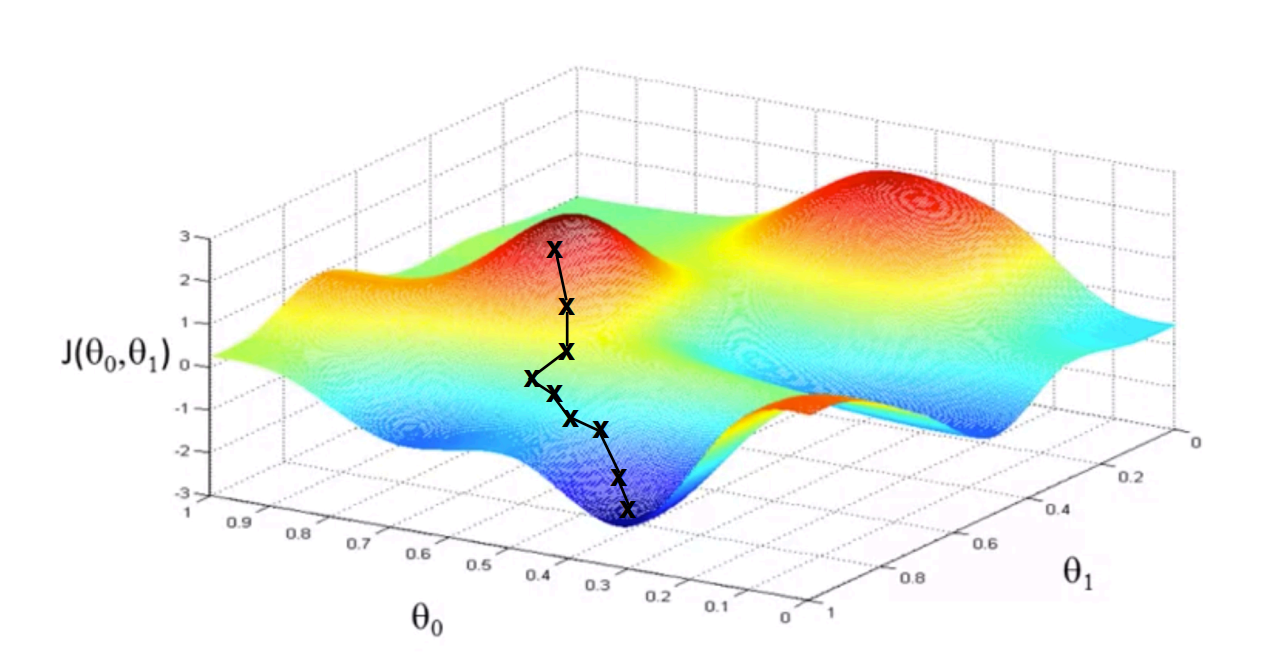
\includegraphics[width=\linewidth]{Images/gradientDescend.png}
  \caption{un esempio grafico per visualizzare cosa acccade.}
  \label{fig:1}
    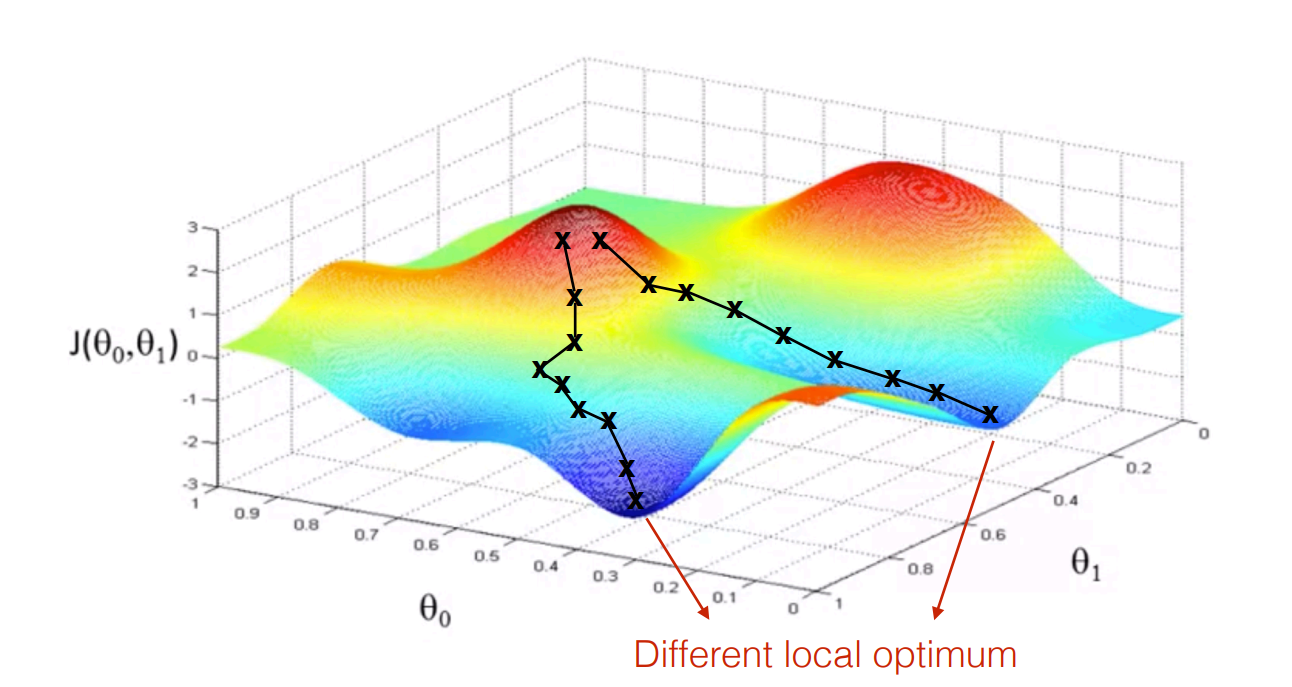
\includegraphics[width=\linewidth]{Images/gradientDescend2.png}
  \caption{Non univocità dell'ottimo trovato.}
  \label{fig:2}
  \end{figure}
  \pagebreak
  \begin{figure}
    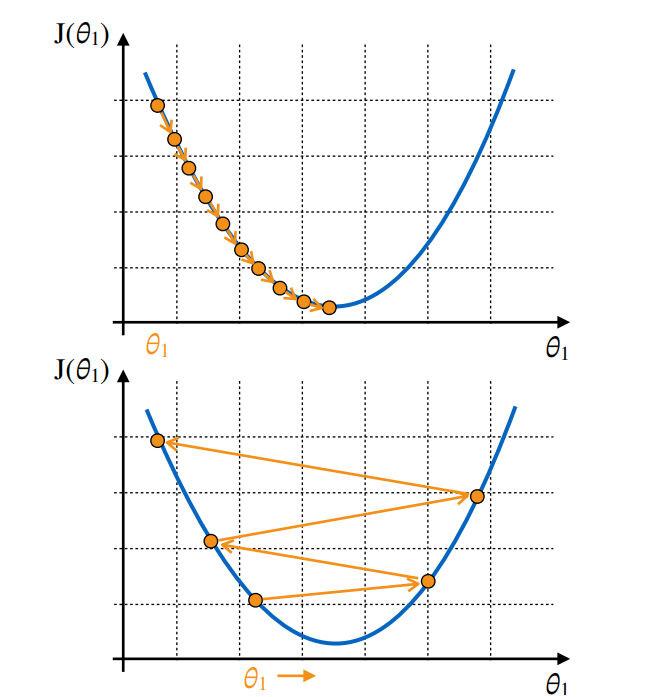
\includegraphics[width=\linewidth]{Images/learningRate.png}
  \caption{Influenza di $\eta$ sulla convergenza.}
  \label{fig:3}
\end{figure}
\pagebreak

\fi

\subsubsection{Features e polynomial regression}
Spesso accade che una funzione lineare non approssimi in maniera accurata i dati.
Perciò possiamo ''duplicare'' una feature \\
\[
\begin{bmatrix}
x_{0} \\
x_{1}  \\
x_{2} \\
\end{bmatrix}
=
\begin{bmatrix}
x^{0} \\
x^{1} \\
x^{2} \\
\end{bmatrix}
\] \\
Questo esempio risulta adatta ad un dataset rappresentabile con una parabola.
Si può usare qualsiasi funzione (radicali, logaritmi, ecc...) e ciò permette maggiore flessibilità

Rimane valida la formula già vista

$$h_{\Theta}(X)=\Theta^{T}X$$

\[
h_{\Theta}(X) = 
\begin{bmatrix}
\Theta_{0} \\
\Theta_{1} \\
\Theta_{2}
\end{bmatrix}^{\!T}
\begin{bmatrix}
x^{0} \\
x^{1} \\
x^{2}
\end{bmatrix}
\]
\subsubsection{Linear classifiers}
Classificazione: \\
serve a determinare a quale categoria specifica un campione appartiene, \\
ad esempio : 
\begin{itemize}
\item il riconoscimento dei numeri
\item riconoscimento delle email di spam

\end{itemize}

La differenza principale tra regressione e classificazione è che la regressione si occupa di calcolare un valore, l'esempio classico è il prezzo delle case di Boston dati alcune caratteristiche, mentre nella classificazione l'output è una classe o etichetta

\begin{itemize}
\item classificazione binaria.\\
2 possibili labels (etichette)
\item Classificazione multi-classe \\
più possibili etichette
\end{itemize}
Con le conoscenze attuali possiamo realizzare la classificazione binaria sfruttando la regressione. \\
\textbf{Classification as regression}
\begin{itemize}
\item Ricordiamo la funzione di regressione 
$$h_{\Theta}(x)=\Theta^{T}x$$
\item fissiamo dei classificatore di soglia

\begin{itemize}
\item se $h_{\Theta}(x) \ge 0,5$ allora predice $y=1$
\item se $h_{\Theta}(x) < 0,5$ allora predice $y=-1$\\
(in base al contesto potremmo avere $y=0$ )
\item Abbiamo usato il -1 così da poter scrivere la funzione di classificazione nel seguente modo:
$$y=sign(h_{\Theta}(x))$$
\item Questa funzione è detta \textbf{linear classifier}, dato che ''imposta'' un confine lineare che separa lo spazio in 2 metà distinte

\item Non sempre è una buona idea, dato che valori estremi potrebbero spostare la soglia e incasinare la classificazione per valori medii
\end{itemize}
\item interpretazione geometrica
\begin{itemize}
\item se lo spazio ha dimensione N, la soglia ha dimensione N-1.
\item spazio a 2 dimensioni, il classificatore è una riga
\item  spazio a 3 dimensioni, la soglia è un piano
\item per spazi con una dimensione di ordine superiore non possiamo visualizzarlo, ma possiamo scriverlo matematicamente

\begin{itemize}
\item $\Theta^{T}x=0$ \\
 è una linea passante attraverso l'origine e ortogonale a $\Theta $ (ritorna uno scalare)
 
 \item  $\Theta^{T}x+\Theta_{0}=0$ \\ shifta la linea di $\Theta_{0}$, viene spesso chiamato ''bias term''
 
 \item perciò la funzione di classificazione è 
 $$sign(h_{\Theta}(x))=sign(\Theta^{T}x+\Theta_{0})$$
\end{itemize}

\end{itemize}

\end{itemize}

\begin{itemize}
\subsubsection{Regolarizzazione}
\item \textbf{Overfitting}: se abbiamo troppe caratteristiche, la funzione ''appresa'' $h_{\Theta}(x)$ potrebbe adattarsi molto bene al set di addestramento, ma fallire nella generalizzazione di nuovi campioni. \\
\item \textbf{Come individuarlo}: se abbiamo troppe caratteristiche e un training set troppo piccolo, potrebbero verificarsi problemi di overfitting.
\item \textbf{Soluzioni}: 
\begin{itemize}
\item Ridurre il numero di caratteristiche durante la model selection
\item Regolarizzazione

\begin{itemize}
\item Mantenere tutte le features/caratteristiche, ma riducendo l'influenza dei parametri $\Theta_{j}$
\item Funziona bene quando abbiamo molte features e ognuna contribuisce un po' a predirre $Y$


\end{itemize}

\end{itemize}
\item Come funziona la \textbf{regolarizzazione}: \\
Supponiamo di voler penalizzare dei $\Theta_{3}$ e $\Theta_{4}$ al fine di renderli molto piccoli.\\
Per fare ciò, ritocchiamo un po' la funzione di costo e alterando così il minimo:
$$ J(\Theta)= \frac{1}{2m} \sum_{i=1}^{m}(h_{\Theta}(x^{(i)})-y^{(i)})^2+1000\Theta_{3}^{2}+1000\Theta_{4}^{2}$$
$$\min_{\Theta} J(\Theta)=\min_{\Theta} \frac{1}{2m} \sum_{i=1}^{m}(h_{\Theta}(x^{(i)})-y^{(i)})^2+1000\Theta_{3}^{2}+1000\Theta_{4}^{2}$$

\item o volendolo scrivere con una sintassi più generica:
$$\min_{\Theta} J(\Theta)=\min_{\Theta} \frac{1}{2m} \sum_{i=1}^{m}(h_{\Theta}(x^{(i)})-y^{(i)})^2+\lambda \sum_{j=1}^{n}\Theta_{j}^{2}$$
Questa modifica permette al \textbf{gradient descend} di ridurre i parametri desiderati

\item Analizzando cosa accade nell'aggiornamento del gradient descend con la nuova funzione di costo:

\begin{itemize}
\item Ripeti fino a convergenza:
$$\Theta_{0}^{j+1}=\Theta_{0}^{j}-\eta \frac{1}{m} \sum_{i=1}^{m}(h_{\Theta^{j}}(x^{(i)})-y^{(i)})x_{0}^{(i)}$$
$$\Theta_{k}^{j+1}=\Theta_{k}^{j}-\eta \frac{1}{m}\sum_{i=1}^{m}(h_{\Theta^{j}}(x^{(i)})-y^{(i)})x_{k}^{(i)}+\frac{\lambda}{m}\Theta_{k}$$
\item analizzando meglio la funzione possiamo scriverla nella seguente maniera:
$$\Theta_{0}^{j+1}=\Theta_{0}^{j}-\eta \frac{1}{m} \sum_{i=1}^{m}(h_{\Theta^{j}}(x^{(i)})-y^{(i)})x_{0}^{(i)}$$
$$\Theta_{k}^{j+1}=\Theta_{k}^{j}(1-\eta \frac{\lambda}{m} )-\eta \frac{1}{m}\sum_{i=1}^{m}(h_{\Theta^{j}}(x^{(i)})-y^{(i)})x_{k}^{(i)}$$

\item Possiamo notare alcune cose molto interessanti:
\begin{itemize}
\item Il primo termine ($\eta \frac{\lambda}{m}$) è poco più piccolo di 1, quindi a riduce il parametro $\Theta_{k}$. \\
Quindi abbiamo:
$$\Theta_{k}^{j}(1-\eta \frac{\lambda}{m} ) < \Theta_{k}^{j}$$ $$ (\approx \Theta_{k}^{j} * 0,99)$$ 
\item Il secondo termine è uguale alla funzione per l'aggiornamento dei $\Theta$ prima che introducessimo la regolarizzazione
$$-\eta \frac{1}{m}\sum_{i=1}^{m}(h_{\Theta^{j}}(x^{(i)})-y^{(i)})x_{k}^{(i)}$$
\end{itemize}

\end{itemize}


\end{itemize}



\subsection{Si descriva in modo accurato il modello di logistic regression, le sue principali caratteristiche
	ed il contributo dei diversi elementi presenti nella funzione di costo. Si riporti inoltre
	una comparazione con il modello di classificazione lineare, evidenziando elementi in comune
	e differenze principali. Infine, si descriva chiaramente la procedura di addestramento
	mediante l’applicazione di gradient descent}

\textbf{attenzione la seguente risposta è da correggere perciò non prendetela per buona}


Classificazione come regressione(o logistic regression, questa cosa è da verificare) :
\begin{itemize}
\item è una funzione di classificazione, ha quindi output binario, ovverro restituisce \textbf{-1} oppure 1\textbf{1}
\item utilizza una funzione trovata tramite regressione lineare e un classificatore a soglia, e per praticità scriviamo la funzione di classificazione come $y = \mathrm{sign}(h_{\Theta}(x)+\Theta_{0})$ dove $\Theta_{0}$ è detto ''bias term'' ed è il classificatore a soglia
\item La funzione di costo è delineata dalle seguenti formule(per praticità mi limito momentaneamente al caso con funzione h lineare):
 \begin{itemize}
 \item la prima funzione è:
  $$h_{\Theta}(x)=\Theta_{0}+\Theta_{1}x$$
 dove i $\Theta_{i}$ rappresentano dei coefficienti che cercano di realizzare una funzione tale che 
 $$h_{\Theta}(x^{(i)})\approx y^{(i)}  \forall i$$
 
 \item La funzione di costo è:
 $$J(\Theta_{0},\Theta_{1})= \frac{1}{2m} \sum_{i=1}^{m}(h_{\Theta}(x^{(i)})-y^{(i)})^2$$
 \item Il nostro obiettivo è minimizzare la funzione di costo
 $$\min_{\Theta_{1}} J(\Theta_{1})$$
 
 \end{itemize}
 
 \item scelta dei parametri $\Theta$ e minimizzazione efficiente della funzione di costo J,
 per fare ciò usiamo la discesa del gradiente o gradient descend
 \begin{itemize}
\item Data una funzione di costo:
$$J(\Theta_{0},......,\Theta_{n})$$
\item facciamo un piccolo ``passo'' nella direzione opposta al gradiente (gradiente moltiplicato per $-1$)
$$\Theta^{(j+1)} = \Theta^{(j)}-\eta \nabla J(\Theta^{(j)})$$
\item $\Theta^{(j)}$ indica l'insieme delle $\Theta_{0},......,\Theta_{n}$ al j esimo passo \\
(\textbf{NB} se l'aggiornamento delle $\theta $ non avviene come operazioni tra vettori, ma considerando ogni $\Theta$ come uno scalare è necessario aggiungere delle variabili temporanee per evitare che i cambiamenti di un $\Theta$ inluenzi anche gli altri)

\item $\eta > 0$ è chiamato \textbf{learning rate}
\item dopo ogni passaggio il gradiente viene rivalutato per il nuovo vettore dei pesi $\Theta^{(j+1)}$ 
\\ il processo si ripete finchè non si raggiunge uno scarto sufficientemente basso (il criterio dello scarto ferma la discesa del gradiente quando la differenza tra il gradiente al passo j e j+1 è prossima a 0 )

\item  \textbf{Nota bene}: la funzione di costo va calcolata sull'interezza dei dati di addestramento gli x e y, \\
in particolare X diventa matrice e Y diventa vettore
$$\nabla J(\Theta)=\frac{1}{m}X^{T}(h_{\Theta}(X)-Y)$$
 \begin{itemize}
\item $X$ è la matrice degli input
\item $X^{T}$ è la matrice degli input trasposta
\item $h_{\Theta}(X)$ è un vettore di tutte le previsioni (calcolate su ogni riga di X)
\item $Y$ è il vettore dei target (i risultati ''reali'' del training set)

\end{itemize}
\item come implementiamo $\nabla J(\Theta^{(j)})$ ovvero il calcolo del gradiente:
eseguiamo l'operazione come segue $\forall i$, ovvero per tutti le caratteristiche (o feature) del nostro training set
$$\Theta^{(j+1)}_{i}=\eta \frac{\partial}{\partial \Theta^{(j)}_{i}} J(Theta^{(j)})$$
 
e ripetiamo tale operazione fino a convergenza

\end{itemize}

\end{itemize}
\subsection{Si descriva in modo dettagliato il modello di logistic regression (con regolarizzazione), le
	sue principali caratteristiche ed il contributo dei diversi elementi presenti nella funzione
	di costo. Si riporti infine una descrizione accurata delle differenze di tale modello rispetto
	ad un semplice classificatore lineare, anche mediante esempi qualitativi}
g
\subsection{Spiegare in dettaglio gli elementi fondamentali del perceptron e, più in generale, delle reti
	neurali. Si riporti inoltre una breve descrizione di come tale modello possa essere esteso
	mediante la realizzazione di un’architettura a più strati, fornendo un esempio che evidenzi
	le differenze/vantaggi di tale architettura}
g
\subsection{Si descriva dettagliatamente la procedura di crossvalidation, motivandone scopo ed utilità,
	e fornendo una chiara descrizione della (corretta) procedura di addestramento di un
	qualunque sistema di machine learning. Si descrivano inoltre i concetti di true error ed
	empirical error e se ne evidenzino le relazioni con la procedura di cross-validation}
g
\subsection{Quali sono i principali paradigmi del machine learning? Se ne riporti una descrizione
	sintetica – chiarendo quali siano le principali differenze – con particolare enfasi per il caso
	del supervised learning. Si distinguano in particolare classificazione e regressione}
g
\subsection{Cosa si intende per “one learning algorithm hypothesis” e come tale ipotesi si relaziona
	con le reti neurali artificiali? Si fornisca inoltre una descrizione esaustiva degli elementi/ingredienti
	principali che permettono la definizione di una rete neurale multistrato}
g
\subsection{Si descriva dettagliatamente la procedura di model selection (aiutandosi con un esempio
	concreto) e si fornisca una chiara giustificazione teorica/concettuale a tale procedura}
g
\subsection{Spiegare in dettaglio gli elementi fondamentali del perceptron e delle reti neurali multistrato.
	Si riporti inoltre un esempio di rete neurale per la realizzazione della porta logica
	NAND (indicando i valori dei parametri e la funzione di attivazione prescelta)}
g
\subsection{Spiegare in dettaglio gli elementi fondamentali del perceptron e, più in generale, delle reti
	neurali. Si riporti inoltre una breve descrizione di come tale modello possa essere esteso
	mediante la realizzazione di un’architettura multistrato, fornendo un esempio che evidenzi
	le diffeerenze ed i vantaggi di tale architettura}
g
\subsection{Spiegare in dettaglio gli elementi fondamentali del perceptron e, più in generale, delle reti
	neurali multistrato, illustrando chiaramente le due fasi di feedforward e backpropagation.
	Si riporti inoltre un esempio di rete neurale per la realizzazione di un semplice operatore
	logico AND, ed uno per la funzione XOR}
g
\section{Seconda parte}
\subsection{Spiegare in dettaglio gli elementi fondamentali di SVM; in particolare: 1) la sua interpretazione geometrica, 2) la funzione di costo, 3) le differenze/similitudini con altri modelli di ML. Infine, si introduca brevemente l’estensione di SVM basata sul kernel trick}
g
\subsection{Si descrivano nel modo più accurato possibile gli alberi di decisione, i loro vantaggi e svantaggi rispetto ad altri modelli (ad es. reti neurali) e si evidenzi il principale inductive bias di tale algoritmo. Si fornisca inoltre un semplice esempio di albero di decisione. Infine, si illustri brevemente l’estensione di tale modello attraverso random forest}
g
\subsection{Si descriva in modo accurato l’algoritmo k-NN, illustrando il ruolo dei principali iperparametri, i vantaggi e le debolezze del modello nei confronti di altri algoritmi affrontati nel corso, e si evidenzi il principale inductive bias di tale algoritmo}
g
\section{Appelli}
\subsection{Si descriva accuratamente un esempio di rete neurale per la realizzazione di un operatore logico XOR (indicando valori dei parametri e funzione di attivazione prescelta); si fornisca inoltre l’analoga soluzione utilizzando un albero di decisione, e si discutano pro e contro delle due soluzioni}
g
\subsection{Si descrivano nel modo più accurato possibile i modelli di linear classification e logistic regression; si evidenzino differenze, vantaggi e svantaggi dell’uno rispetto all’altro. Si descriva infine il processo di apprendimento tramite gradient descent e le rispettive funzioni di costo, motivando in modo adeguato la particolare forma utilizzata in entrambi i casi.}
g
\subsection{Si descriva accuratamente un esempio di rete neurale per la realizzazione di un operatore logico AND, ed uno per la funzione OR (indicando valori dei parametri e funzione di attivazione prescelta). Si riporti infine un esempio di rete neruale per lo XNOR}
g
\subsection{Si descrivano nel modo più accurato possibile il modello di regressione lineare e la sua “estensione” al problema di classificazione. Infine, si compari il modello di classificazione lineare con quello di logistic regression, evidenziando le principali differenze}
g
\end{document}